\documentclass[12pt]{article}

\usepackage{sbc-template}
\usepackage{graphicx,url}
\usepackage[latin1,utf8]{inputenc}
\usepackage[brazil]{babel}
\usepackage[nonewpage]{imakeidx}
%\usepackage{indentfirst} % Pacote para indentar o primeiro parágrafo depois de um título

\sloppy

\makeindex[columns = 1]%,title= ]

\title{Documentos de Requisitos\\ Aplicativo para distribuição de informações}

\author{João Victor F. Consonni\inst{1}, Victor H. C. Leite\inst{1}, Matheus Ferreira\inst{1}, \\Matheus Milani\inst{1}, Artur L. Silva\inst{1}, Gustavo F. Fogolin\inst{1}, \\Bruno J. M. de Camargo\inst{1}, Danilo B. Cardoso\inst{1}, Daniel P. Cinalli\inst{1}, Lucas K. Kurokawa\inst{1}}

\address{Centro de Matemática, Cognição e Computação\\ Universidade Federal do ABC
  (UFABC)\\
Av. dos Estados, 5001 - Bangú -- Santo André -- SP -- Brazil
  \email{\{jconsonni, victor.costa, matheus.ferreira, milani.matheus, }
  \email{artur.lazarini, gustavo.fogolin, bruno.camargo,}
  \email{danilo.c, dpcinalli, kenzo.kurokawa\}@aluno.ufabc.edu.br}
}

\begin{document} 

\maketitle

\begin{abstract} 
  Identifying system requirements is key to guiding all subsequent stages of project development. Therefore, this document aims to identify and specify the requirements of the system, describing, in detail, the elements involved, in what context they are inserted and how they will be approached by the proposed application.
\end{abstract}

\begin{resumo} 
   A identificação dos requisitos do sistema é fundamental para guiar todas as etapas seguintes do desenvolvimento do projeto. Por isso, este documento visa identificar e especificar os requisitos do sistema, descrevendo, de forma detalhada, os elementos envolvidos, em que contexto estão inseridos e como serão abordados pela aplicação proposta.
\end{resumo}
\section{Introdução}
\subsection{Propósito do documento de requisitos}
%Especificar objetivos e público-alvo do DR
A fim de compreender as necessidades e restrições da aplicação, utilizamos o conceito de requisitos para documentar as características e funcionalidades do sistema. Este documento visa definir os requisitos necessários para a criação de um aplicativo mobile colaborativo, voltado para a melhoria da gestão de risco de desastres ambientais, de forma a informar seus usuários sobre as condições ambientais em suas proximidades. 

\subsection{Escopo do produto}
%Explicitar o que o produto faz (e o que não faz).
%Descrever a aplicação (pontos relevantes, objetivos e metas)
O aplicativo será um meio de compartilhamento de informações, onde os usuários terão a possibilidade de publicarem e serem informados sobre a presença de incidentes, os visualizando em balões, em um mapa que abrange todo o território nacional. Será possível ser notificado de incidentes perto de sua localização e outros locais definidos pelos usuários. 

Para garantir a confiabilidade do aplicativo, usuários próximos ao local de um incidente indicado por outro usuário, serão requisitados a confirmar a veracidade desta informação. Também será feita a leitura de diversos sensores que podem indicar a presença de incidentes, como de pluviômetros e sismógrafos, que também serão disponibilizados no mapa.

O objetivo do aplicativo é informar as pessoas e assim possibilitar a diminuição da quantidade de vítimas desses incidentes causados pela chuva, proporcionando a possibilidade de evitar esses pontos. O aplicativo, no entanto, não poderá emitir alertas com base nos incidentes informados por usuários, já que essa emissão pode ser realizada apenas pela Defesa Civil.

\subsection{Definições, acrônimos e abreviações}\label{subsec:Defs}
\begin{itemize}
    \item [DR]-Documento de requisito.
    \item [RNF]-Requisito não funcional.
    \item [RF]-Requisito funcional.
    \item [RD]-Requisito de domínio.
    \item [TP]-Tela principal.
    \item [CI]-Cadastro de incidente.
    \item [EI]-Edição de incidente.
    \item [RI]-Remoção de incidente.
    \item [VI]-Visualização de incidente.\index{VI - Visualização de incidente}
\end{itemize}
\index{DR - Documento de requisito}
\index{RFN - Requisito não funcional}
\index{RF - Requisito funcional}
\index{RD - Requisito de domínio}
\index{TP - Tela principal}
\index{CR - Cadastro de incidente}
\index{EI - Edição de incidente}
\index{RI - Remoção de incidente}

\subsection{Referências} \index{Referências}

\subsection{Visão geral do documento de requisitos}
%Descrever a estrutura/organização do restante do DR
O DR foi estruturado com base no padrão IEEE 830 \cite{ieee1994ieee}, com algumas modificações, sendo elas:
%talvez mude, entao preencher depois
\begin{itemize}
    \item Requisitos de Desempenho e Requisitos Lógicos de Banco de Dados dentro da seção \ref{subsec:RequisitosNaoFuncionais}, como requisitos não funcionais;
    \item Restrições de Projeto estarão na seção \ref{subsec:RequisitosDominio}, como requisitos de domínio;
\end{itemize}

Na seção \ref{subsec:RequisitosFuncionais}, os requisitos funcionais foram divididos nas seguintes categorias:
\begin{itemize}
    \item Tela Inicial;
    \item Tela Principal;
    \item Cadastro de Incidente;
    \item Edição de Incidente;
    \item Remoção de Incidente;
    \item Visualização de incidente.
\end{itemize}

Por convenção, os requisitos devem ser identificados com um identificador único, de acordo com a seção \ref{subsec:Defs}. A numeração inicia com o identificador e prossegue sendo incrementada à medida que forem surgindo novos requisitos, por exemplo RF01 (Requisito Funcional numero 01).

\section{Descrição Geral}
\subsection{Perspectiva do Produto}
O sistema consiste em um aplicativo de celular que opere nos sistemas operacionais Android e iOS. O objetivo do aplicativo é criar uma estrutura colaborativa para melhorar a gestão do risco de desastres ambientais, em nível nacional, com ênfase para enchentes e alagamentos causados por chuvas.

O aplicativo busca criar um canal de comunicação centralizado para que usuários geograficamente dispersos possam consultar a situação ambiental em regiões de interesse, assim como compartilhar o status de sua região atual, de forma a auxiliar os demais usuários na sua tomada de decisão. 

O aplicativo se comunica com um servidor remoto que opera um banco de dados que centraliza informações reportadas pelos usuários, assim como dados ambientais, estruturais e meteorológicos captados por entidades responsáveis. 
\subsection{Funções do Produto (Requisitos do cliente)} \index{Requisitos do Cliente}
\begin{enumerate}
    \item [RC01] As publicações dos usuários devem ser públicas, qualquer outro usuário deve pode vê-las.
    \item [RC02] O aplicativo deverá permitir aos usuários reportar as condições ambientais correntes em sua região.
    \item [RC03] O aplicativo deverá permitir que as publicações feitas possam ser compartilhadas externamente com o aplicativo Whatsapp.
    \item [RC04] O aplicativo deverá permitir que as publicações feitas possam ser compartilhadas externamente com o aplicativo Outlook.
    \item [RC05] O aplicativo deverá permitir que as publicações feitas possam ser compartilhadas externamente com o aplicativo Gmail.
    \item [RC06] O aplicativo deverá permitir que as publicações feitas possam ser compartilhadas externamente com o aplicativo Facebook.
    \item [RC07] O aplicativo deverá permitir que as publicações feitas possam ser compartilhadas externamente com o aplicativo Twitter.
    \item [RC08] O aplicativo deverá consultar meios tradicionais de informação, como estações hidrológicas, pluviômetros e sismógrafos para gerar alertas aos usuários com previsões de mau tempo.
    \item [RC09] O aplicativo deverá permitir ao usuário visualizar as condições ambientais de uma região de seu interesse.
    \item [RC10] O aplicativo deverá repassar avisos emitidos pela defesa civil para os usuários em área de risco.
    \item [RC11] Usuários devem poder configurar regiões para as quais gostaria de receber alertas da defesa civil.
    \item [RC12] Juntamente com o aviso de risco o aplicativo deverá sugerir possíveis ações que o indivíduo possa tomar com objetivo de minimizar a vulnerabilidade do cidadão aos possíveis impactos do incidente ambiental.
    \item [RC13] O aplicativo deverá solicitar aos usuários que confirmem as condições ambientais reportadas por outros usuários, para a sua região atual.
    \item [RC14] O produto deve ter potencial de expansão para outras áreas potencialmente sujeita aos riscos abordados.
    \item [RC15] O aplicativo deverá permitir que os usuários atualizem o status de incidentes, incluindo mais informações ou comentários por texto.
    \item [RC16] O aplicativo deverá permitir que os usuários atualizem o status de incidentes enviando imagens.
    \item [RC17] O aplicativo deverá permitir que o usuário cadastre trajetos que costuma fazer para que, caso ocorra incidentes no percurso, receba um aviso.
    \item [RC18] Quando requisitado, o aplicativo deverá fornecer ao usuário informações de contato de emergência e de serviços públicos.
    \item [RC19] O aplicativo deverá permitir que o usuário remova um incidente reportado erroneamente por ele.
    \item [RC20] O aplicativo deverá permitir ao usuário a criação de um login com senha para identificação única no sistema.
    \item [RC21] O aplicativo deverá permitir ao usuário a realização de login por meio de conexão pelas redes sociais Facebook e Twitter ou pelos e-mails Gmail, Hotmail ou Outlook.
    \item [RC22] O aplicativo deve permitir que um usuário cadastre uma senha para sua conta de usuário.
    \item [RC23] O aplicativo deve permitir o usuário alterar a sua senha.
    \item [RC24] O aplicativo deve permitir o usuário a logar usando biometria.
    
    
\end{enumerate}

\subsection{Características do Usuário}
O aplicativo será destinado a população geral brasileira, com o recorte dos 68\% dessa população indicados usuários de redes móveis no Brasil\cite{IBGEPNAD}. O grupo é caracterizado digitalmente por um maior uso do sistema operacional Android (91\%) seguido pelo iOS (7\%)(Figura 1.a). Dentro dos aplicativos de maior relevância na utilização estão Whatsapp (48\%), Facebook (8\%) e Instagram (6\%), com destaque ainda à aplicativos da Google LLC (Google e Youtube com 2\% cada)(Figura 1.b).

\begin{figure}[!htb]
\centering
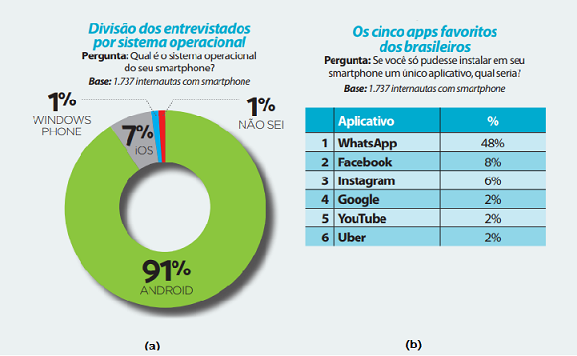
\includegraphics{caract_user}
\caption{Caracterização digital do usuário: (a)  divisão por sistema operacional e (b) aplicativos de referência. Adaptado: Opinion Box. 2018}
\label{Rotulo}
\end{figure}

Para a instalação de novos aplicativos, existe uma alta volatilidade, onde onde 38\% dos usuários desinstala aplicativos após 24 horas da instalação, justificada pela falta de espaço de armazenamento nos dispositivos \cite{Obox}. Na perspectiva de conectividade dessa população existe a dominância de planos pré-pagos \cite{Obox}. 


\subsection{Restrições}

Das restrições legais:

\begin{enumerate}
    \item  Deve-se seguir as diretrizes da lei  lei federal No12.608/12 \cite{leiPNSB} que restringe a emissão de alertas de desastres aos órgãos públicos repensáveis.
\end{enumerate}

Das restrições e políticas de uso das APIs e SDKs para logins e compartilhamento de informações:
\begin{enumerate}
\item Utilizar botões textos de acordo com a identidade visual e padrões de visualização definidos pela marca associada \cite{FACEBOOKDEV} \cite{TWITTERDEV}\cite{GOOGLEDEV}.
\item Ter opção visível para sair do serviço dentro da aplicação \cite{FACEBOOKDEV}\cite{TWITTERDEV}.
\item Requirir apenas as permissões e dados necessários ao uso da aplicação \cite{FACEBOOKDEV}\cite{TWITTERDEV}\cite{GOOGLEDEV}  .
\item Caso a publicação no Twitter tenha mais de 140 caracteres, é necessário a inclusão de um link que encaminhe diretamente para a página associada à publicação, sem sites intermediários \cite{TWITTERDEV}.
\item Para publicações no Facebook deve-se pedir a permissão de publicação ao usuário junto de uma pré-visualização da publicação \cite{FACEBOOKDEV}.
\end{enumerate}

As APIs de login da Microsoft não apontam diretrizes quem restringem o  login e compartilhamentos dentro da aplicação, excluindo as diretrizes gerais de desenvolvimento e manutenção do perfil de desenvolvedor.
 
\subsection{Suposições e dependências}

Para o uso das API de cada fornecedor é necessário a criação de um perfil de desenvolvedor associado, seguindo o processo e documentação determinado por cada fornecedor. 
%definições para usuário baseado nos dados sobre SOs, aplicativos para criações de contas e uso de dados
%dependências de contas de desenvolvimento para APIs e SDKs

\section{Requisitos Específicos}
%\subsection{Interfaces Externas}
\subsection{Requisitos Funcionais}
\label{subsec:RequisitosFuncionais}

\subsubsection{Tela inicial} \index{Tela inicial}
\begin{enumerate}
    \item [TI01] A tela inicial deve conter uma caixa de Login, com usuário e senha.
    \item [TI02] A tela inicial deve conter opções para Login rápido por meio do Facebook, Twitter, Outlook, Hotmail ou Google.
    \item [TI03] A tela inicial deve conter opção de lembrar a senha.
    \item [TI04] A tela inicial deve conter opção de logar por biometria.
    \item [TI05] A tela inicial deve conter opção para novo cadastro de usuário.
    \item [TI06] O cadastro de usuário deve exigir um nome de login, uma senha, um e-mail e a localização da residência.
\end{enumerate}

\subsubsection{Tela Principal}
\begin{enumerate}
    \item [TP01] A tela principal do aplicativo deverá conter o mapa do Brasil com foco na região de moradia cadastrada para o usuário ou prioritariamente a região indicada pelo GPS do usuário se este estiver ativo.
    \item [TP02] No mapa deverão estar dispostos balões representando as publicações das pessoas.
    \item [TP03] Os balões deverão estar localizados no mapa no local que o incidente relatado representado pelo balão ocorreu.
    \item [TP04] Deve ser apresentado um máximo de 10 balões na tela.
    \item [TP05] Quando houver mais balões do que o limite máximo, os balões concentrados em uma região devem ser representados por um balão contendo o número de balões presentes naquela localidade.
    \item [TP06] Conforme for dado zoom na tela, os balões que representam um determinado número de balões deve ser expandido em mais de um balão sempre procurando respeitar o limite máximo de balões na tela.
    \item [TP07] O balão não selecionado deve possuir cor referente à situação do local (exemplo: verde para "OK", amarelo para "atenção", vermelho para "risco ou perigo").
    \item [TP08] Caso a publicação não tenha uma imagem anexada pelo autor da publicação, deverá ser apresentado a classificação do incidente conforme apêndice A feita pelo autor da publicação.
    \item [TP09] Quando um balão for selecionado deve ser apresentada a tela de visualização de incidente.
    \item [TP10] A tela principal deve possuir filtros nos balões que serão apresentados. Filtro por tempo desde a publicação, cidade do incidente e classificação do incidente conforme apêndice A.
    \item [TP11] A tela principal deve possuir uma opção para iniciar o cadastro de um incidente.

\end{enumerate}

\subsubsection{Cadastro de Incidente}
\begin{enumerate}
    \item [CI01] No cadastro de incidente o usuário deve fornecer obrigatoriamente uma descrição do incidente, a localização do incidente e uma classificação do incidente de acordo com o Apêndice A.
    \item [CI02] O autor de uma publicação deve estar com o GPS ligado durante o cadastro de um incidente.
    \item [CI03] A localização do incidente deve estar limitada a um raio de 300 metros do usuário, de forma que apenas usuários que estejam presenciando o incidente possam reporta-lo.
    \item [CI04] No cadastro do incidente, o usuário poderá fornecer, se desejar, uma foto do incidente.
    \item [CI05] Ao ser cadastrado, o incidente deverá ficar disponível para público e aberto para avaliação de outros usuários.
    \item [CI06] Deve haver um limite de 3 fotos por publicação por autor.
    \item [CI07] Devem ser aceitos somente fotos com extensão .png e .jpg.
    \item [CI08] A tela de cadastro de incidente deverá ter como opção um ícone para abrir a câmera e tirar uma foto para anexo na publicação.
    \item [CI09] O aplicativo deve evitar novos Incidentes com as mesmas características quando os balões estiverem muito próximos (300 metros ou menos).% Evitar para um mesmo usuário ou para todos? Não está claro. Acredito que o melhor seja para o mesmo usuário. Novos posts de outros usuários podem eventualmente ser agrupados sobre um único incidente com maior grau de confiabilidade da informação.
    \item [CI10] Um balão de um novo incidente deverá ser mostrado no mapa com a coloração vermelha.
\end{enumerate}
\subsubsection{Edição de Incidente}
\begin{enumerate}
    \item [EI01] Apenas o autor da publicação poderá editar uma publicação.
    \item [EI02] Será permitido a edição de uma publicação apenas se a publicação não possuir comentários de outro usuário que não o autor.
    \item [EI03] O autor poderá editar a descrição do incidente, a classificação do incidente e as fotos em anexo. 
\end{enumerate}
\subsubsection{Remoção de Incidente}
\begin{enumerate}
    \item [RI01] Após receber 10 avaliações de Incidente Passado, o balão que representa a publicação deverá ficar com cor verde.
    \item [RI02] Passadas 8 horas que o balão está com coloração verde, o balão deverá deixar de ser mostrado no mapa.
    %Apenas uma avaliação informando que o incidente passou é suficiente para eliminar o balão? A ideia é ser colaborativo e dinâmico: a medida que o tempo for passando, as pessoas irão começar a informar que a situação está normalizando. Depois de um número x de pessoas informarem que está tudo bem, o balão fica verde e, após y horas de normalização o balão some. Acho importante que x seja maior que 10, ou 20 e que y seja pelo menos 8 horas, pois uma pessoa pode querer saber se está tudo bem e ela já pode ir/sair pra/de casa (o balão verde confirma isso)
\end{enumerate}
\subsubsection{Visualização de Incidente}
\begin{enumerate}
    \item [VI01] A tela de visualização de incidente deverá ser apresentada ao selecionar uma publicação no mapa da tela principal.
    \item [VI02] A tela de visualização de incidente deverá apresentar uma opção para retornar ao mapa da tela principal.
    \item [VI03] A tela de visualização de incidente deverá mostrar o texto do autor relatando o incidente, se houver.
    \item [VI04] A tela de visualização de incidente deverá mostrar a(s) foto(s) anexa(s) pelo autor relatando o incidente, se houver.
    \item [VI05] A tela de visualização de incidente deverá mostrar a classificação do incidente.
    \item [VI06] A tela de visualização de incidente deverá mostrar os comentários de outros usuários, se houver.
    \item [VI07] Caso não haja comentários ou fotos em anexo em uma publicação, deverá ser apresentado uma mensagem informando explicitamente que não há tal item na publicação.
    \item [VI08] A tela de visualização de incidente deverá apresentar opções para comentar a publicação com mensagens de texto ou fotos.
    \item [VI09] Para o autor da publicação, e apenas para ele, a tela de visualização de incidente deverá apresentar a opção de editar a publicação.
    \item [VI10] Na tela de visualização de incidente os usuários deverão ter a opção de avaliar um incidente como "Incidente Presente" e "Incidente Passado".
\end{enumerate}

\subsection{Requisitos Não Funcionais}
\label{subsec:RequisitosNaoFuncionais}
\subsubsection{Requisitos do Produto}
\begin{enumerate}
% Acredito que faltaram requisitos de confiabilidade (disponibilidade 24/7), tempo de recupereção.
    \item [RNF01] O aplicativo deve atualizar a sua tela principal a cada 30 segundos, ou ao ser solicitado pelo usuário.%edit
    \item [RNF02] O sistema de localização deve ter precisão de até 20 metros.%edit
    \item [RNF03] O tamanho máximo final do instalável deve ser 100mb.%edit
    \item [RNF04] O tamanho máximo de aplicativo instalado deve ser 200mb.%edit
    \item [RNF05] Ao primeiro uso do aplicativo será apresentado ao usuário um pequeno tutorial do aplicativo.%edit apesar de debativel, não seria melhor um tutorial pulável? como quando uma pessoa reinstala o aplicativo.
    \item [RNF06] O sistema deve possuir explicação e informações para usuários leigos.%edit aqui tambem acho que seria melhor o usuário poder selecionar se ele quer desativar as dicas, por ser dificil definir quem é leigo ou não.
    \item [RNF07] O aplicativo deve ser compatível com sistemas Android 5.0 ou superior e com iOS 10.0 ou superior.
    \item [RNF08] O sistema deverá ter disponibilidade mínima de 95\% do tempo.%edit
    \item [RNF09] O sistema deverá ser desenvolvido na linguagem Java.%edit
    \item [RNF10] O sistema deve ter uma API para se comunicar com Google Maps.%edit
    \item [RNF11] O sistema deve ter um banco de dados estruturado.%Banco relacional?
\end{enumerate}
\subsubsection{Requisitos Organizacionais}
\begin{enumerate}
    \item [RNF12] Deve ser utilizado o Modelo de Desenvolvimento Scrum.%Isso é um requisito do produto?
    \item [RNF13] Deve ser desenvolvido diagramas na Linguagem UML para estruturação da aplicação.%Isso é um requisito do produto?
    \item [RNF14] O sistema deve ser estruturado de acordo com a Programação Orientada a Objetos.%edit
\end{enumerate}
\subsubsection{Requisitos Externos}
\begin{enumerate}
    \item [RNF15] O aplicativo não pode emitir alertas de incidentes naturais.%edit alterado para alertas climaticos para nao confundir com alertas de smartphone.
    \item [RNF16] O aplicativo deve retransmitir alertas da defesa civil.%edit
    \item [RNF17] O local em tempo real dos usuários deve ser disponível apenas ao sistema.%edit
    \item [RNF18] O usuário pode escolher quais dados pessoais deseja compartilhar.%edit
\end{enumerate}

\subsection{Requisitos de Domínio}
\label{subsec:RequisitosDominio}
\begin{enumerate}
    \item [RD01] Referindo-se ao RNF15, com base na lei federal Nº 12.608/12\cite{PNPDEC}, não cabe a instituições privadas produzir alertas antecipando desastres naturais, sendo esta atividade atribuída aos órgãos públicos responsáveis.
    \item [RD02] As eventuais notificações próprias que o aplicativo enviará ao usuário devem relatar as condições atuais da região onde o usuário está situado, para que estas notificações não sobreponham os possíveis alertas oficiais, mencionados em RD01.
    \item [RD03] Requisitos funcionais e não funcionais que dependem, tratam, manuseiam ou armazenam dados do usuário, sensíveis ou não, devem garantir que critérios de proteção e privacidade de dados definidos na lei federal Nº 13.709/18. \cite{PrivDados}
    \item [RD04] Referir-se à convenção de classificação de intensidade de chuva, disponibilizado pelo ClimaTempo \cite{ClimaTempo}, para o mapeamento da entrada o usuário ao relatar uma condição climática.
    \item [RD05] O cálculo que classificara a intensidade de chuva em uma região deve considerar os dados fornecidos pelos usuários, em uma média das intensidades descritas nos últimos 10 minutos, e os dados externos obtidos através de parceiros ou equipamentos meteorológicos.%(?)
    \item [RD06] Para que uma área seja classificada como possivelmente alagada, deverá existir ao menos relatos recentes relacionados a inundações em um raio de 30m.%(?)
    \item [RD07] As classificações dos incidentes devem decorrer do manual de Classificação e Codificação Brasileira de Desastres. \cite{COBRADE}
    \item [RD08] Em decorrência do Art. 252 do Código de Trânsito Brasileiro \cite{transito}, que classifica o uso de aparelhos moveis durante a condução de um automóveis como infração, o usuário deverá confirmar que não está dirigindo ao utilizar o aplicativo.
    \item [RD09] Uma região será considerada de risco ou perigo, caso existam múltiplos relatos recentes de chuva forte nos últimos 30 minutos ou caso exista uma área já classificada como alagada.
    \item [RD10] Uma região será considerada de possível risco (representando o nível 'Atenção', citado em TP07) caso existam no mínimo um relato recentes de chuva forte nos últimos 30 minutos ou caso exista múltiplos relatos recentes de chuva moderada na ultima hora.
\end{enumerate}

\subsection{Organização}
Os requisitos de usuário foram apresentados na seção 2.2, enquanto que os requisitos de sistema foram organizados no capítulo 3 ao longo de três seções, uma para cada um dos três tipos de requisitos de produto. Dentro de cada seção, foram criadas subseções, quando pertinente, buscando deixar o documento mais claro e modularizado.

\section{Discussão}

Durante a elaboração do documento de requisitos foi possível perceber o quanto este é importante para o projeto de um software, pois ele irá nortear o restante do trabalho feito pela equipe. É essencial que ele seja bem elaborado e pensando, considerando todos os fatores da aplicação, de seus usuários e das características do desenvolvimento. Além disso, foi possível perceber o quanto se pode aprofundar nessa questão, pois muitos requisitos que a princípio parecem bem definidos, quando analisados no contexto da aplicação podem ser redefinidos ou ainda gerar novos requisitos.

Sabemos que em metodologias ágeis de desenvolvimento como o Scrum há uma contínua atualização dos requisitos, possibilitando um aperfeiçoamento da precisão destes, onde se pode encontrar requisitos conflitantes ou redundantes e reformulá-los, sempre visando um software de acordo com o que o cliente deseja dentro dos limites técnicos.



\section{Conclusão}
Documentar os requisitos foi uma forma de organizar os serviços fornecidos pelo sistema, que ao fim refletem as necessidades do usuário. Com a divisão dos requisitos em funcionais e não funcionais, por exemplo, acabamos por perceber como a engenharia de requisitos trabalha para extrair essas informações que são de extrema importância para o desenvolvimento de uma aplicação.

Adequado a nosso contexto, utilizamos como base para nosso documento de requisitos o padrão IEEE-830. Com o levantamento dessas informações, foi possível observar a importância desse estágio com o restante do projeto, mesmo que ainda estejamos em fase inicial. Entendemos os requisitos como parte integrante do planejamento de trabalho, e que sendo bem feito irá possibilitar maior organização e menores duvidas sobre a funcionalidade do aplicativo.

Aproveitando para analisar o documento na visão de metodologia de trabalho, os requisitos facilitam o trabalho no modelo ágil, possibilitando entender melhor as necessidades dos usuários e também como realizar a divisão das entregas nas Sprints, portanto gerando maior valor a nosso cliente.

\section{Informações de Apoio}
\subsection{Apêndices}
\subsubsection{Apêndice A - Classificações de incidentes}
Os incidentes cadastrados deverão receber uma das seguintes classificações:
\begin{enumerate}
    \item Enchente
    \item Tempestade
    \item Chuva
    \item Falta de luz
    \item Tornado
    \item Terremoto
    \item Granizo
    \item Neve
    
\end{enumerate}

\subsubsection{Apêndice B - Descrever como o processo de Scrum foi seguido pela equipe}

Estamos com uma identidade maior como equipe, o que facilita bastante a transparência de informações e comunicação entre todos. Tudo isso acaba facilitando nosso trabalho baseado na metodologia Scrum, nos tornando ágeis e adeptos cada vez mais a mudanças no projeto. Justamente sobre mudanças, acabamos por alterar o escopo do projeto, muito disto, viabilizado pelo método ágil.

Ferramentas de trabalho ágeis foram incorporadas nesta segunda Sprint, afim de termos mais indicadores e melhorar a organização da equipe para as demais Sprints que virão. Por exemplo, utilizamos o Poker Planning para pontuar os cards criados, e a equipe ter uma visão maior de complexidade das atividades e divisão delas entre o grupo. Começamos a utilizar o critério de aceite definido pelo Product Owner dentro dos Cards.

Ao final dessa segunda Sprint, nos sentimos mais alinhados ao método ágil Scrum, a dinamicidade do projeto ajuda a nos moldar como equipe ágil. Refinamos, medimos e mudamos ao decorrer da Sprint atual, tudo isso graças à identidade que estamos criando, conforme dito anteriormente. Como possíveis melhorias, teremos que melhorar o refinamento de atividades para adequação à próxima Sprint, e aproveitar o momento de Planning para sairmos com as tarefas divididas entre os membros do time.

\bibliographystyle{sbc}
\bibliography{entrega_02_01}

\end{document}
